%%%%%%%%%%%%%%%%%%%%%%%%%%%%%%%%%%%%%%%%%%%%%%%%%%%%
\section{アルゴリズム}

\subsection{手法概要}

Apriori-Window は、Apriori の反単調性~\cite{agrawal1994fast}を
スライディングウィンドウ局所頻度評価に適用した厳密列挙アルゴリズムである。
入力はイベントストリーム、ウィンドウ幅 $W$、閾値 $\theta$、
およびスキャン頻度 $\Delta$ であり、
出力は全密集パターン $X$ とその密集区間集合 $\mathrm{DI}(X)$ の列挙である。

アルゴリズムはアイテムセットサイズ $k = 1$ から始まり、
サイズ $k$ の密集パターン集合 $L_k$ からサイズ $k{+}1$ の候補を生成し、
各候補の密集区間を計算することを繰り返す。
各アイテムセット $X$ の密集区間計算では、
ウィンドウ $[l, l{+}W]$ 内の $X$ の出現数をカウントしながら左から右へスライドさせる。
このスライド幅を動的に調整する Scan Stride Skipping により、
不要なスキャンを省いて計算コストを削減する。
さらに Apriori の反単調性を用いた候補区間の枝刈り、
Apriori Interval Pruning により探索空間を絞り込む。

スキャンは $\Delta$ 秒ごとにトリガーされ、
直前の走査終端位置を引き継いで新着イベントを対象に走査を継続する。
$\Delta$ を小さくするほどリアルタイム性が向上し、
大きくするほど Scan Stride Skipping の恩恵によりスキャン回数が減り計算コストが下がる。

アルゴリズム~\ref{alg:aw} に全体手順を示す。
$\mathrm{Scan}$ は Scan Stride Skipping を適用した単調スキャンであり、
候補スキャン範囲 $R_X$ は Apriori Interval Pruning で計算する。

\begin{algorithm}[t]
\caption{Apriori-Window（単一スキャン）}\label{alg:aw}
\begin{algorithmic}[1]
\Require $\mathit{occ}$：アイテム$\to$発生位置列マップ；$W$；$\theta$
\Ensure $F$：パターン$\to$密集区間集合マップ
\State $F \leftarrow \emptyset$；$L_1 \leftarrow \emptyset$
\For{$x \in \mathrm{sorted}(\mathrm{keys}(\mathit{occ}))$}
  \State $\mathrm{DI}(x) \leftarrow \mathrm{Scan}(\mathit{occ}(x),\, W,\, \theta,\, \text{全範囲})$
  \If{$\mathrm{DI}(x) \neq \emptyset$}
    \State $F[\{x\}] \leftarrow \mathrm{DI}(x)$；$L_1 \leftarrow L_1 \cup \{\{x\}\}$
  \EndIf
\EndFor
\State $k \leftarrow 2$；$L_p \leftarrow L_1$
\While{$L_p \neq \emptyset$}
  \State $C_k \leftarrow \mathrm{AprioriJoin}(L_p)$
  \State $L_k \leftarrow \emptyset$
  \For{$X \in C_k$}
    \State $\mathit{occ}(X) \leftarrow \bigcap_{x \in X} \mathit{occ}(x)$
    \If{$\mathit{occ}(X) = \emptyset$} \textbf{continue} \EndIf
    \State $R_X \leftarrow \mathrm{cand}(X)$
    \If{$R_X = \emptyset$} \textbf{continue} \EndIf
    \State $\mathrm{DI}(X) \leftarrow \mathrm{Scan}(\mathit{occ}(X),\, W,\, \theta,\, R_X)$
    \If{$\mathrm{DI}(X) \neq \emptyset$}
      \State $F[X] \leftarrow \mathrm{DI}(X)$；$L_k \leftarrow L_k \cup \{X\}$
    \EndIf
  \EndFor
  \State $L_p \leftarrow L_k$；$k \leftarrow k + 1$
\EndWhile
\State \Return $F$
\end{algorithmic}
\end{algorithm}

\subsection{Scan Stride Skipping}

$l$ を毎ステップ1ずつインクリメントするナイーブな方法は非効率である。
そのため、スキャンせずとも確実に密集・非密集が判定できる区間はスキャンをスキップする。

固定アイテムセット $X$ に対し、$\mathit{occ}(X)$ を $X$ が出現するタイムスタンプのソート済みリストとする。
ウィンドウ $[l, l{+}W]$ 内のアイテムセット $X$ の出現数を $c$ とする。
$c$ と $\theta$ の大小に応じた2分岐のストライドにより $l$ を更新することで、確実に密集・非密集が判定できる区間はスキャンをスキップする。（図~\ref{fig:scan_stride}）。

\textbf{密集フェーズ}（$c \geq \theta$）：
$i_{\mathrm{start}}$ をウィンドウ内の最初の出現インデックスとする。
ウィンドウを右にスライドさせて、余剰 $c - \theta$ の分がウィンドウ外に出たとしても、閾値以上であることは保証される。
したがって、区間 $[l,\, \mathit{occ}(X)[i_{\mathrm{start}} + c - \theta] + W]$ を密集区間として出力したうえで、
以下のように$l$ を更新し、次のスキャンを開始する：
\begin{equation}\label{eq:stride_dense}
  l \leftarrow \mathit{occ}(X)[i_{\mathrm{start}} + c - \theta] + 1.
\end{equation}

\textbf{非密集フェーズ}（$c < \theta$）：
$i_{\mathrm{end}}$ をウィンドウ直後の最初の出現インデックスとする。
ウィンドウ内の出現数は $c < \theta$ であり、次に密集となりうる最小の左端は
不足分 $\theta - c$ 個の出現を新たに取り込む位置である。
したがって、以下のように $l$ をジャンプさせ、次のスキャンを開始する：
\begin{equation}\label{eq:stride_sparse}
  l \leftarrow \mathit{occ}(X)[i_{\mathrm{end}} + (\theta - c) - 1] - W.
\end{equation}

両フェーズの正当性は付録~B（補題~\ref{lem:stride_dense}，補題~\ref{lem:stride_sparse}）に示す。

\begin{figure}[t]
\centering
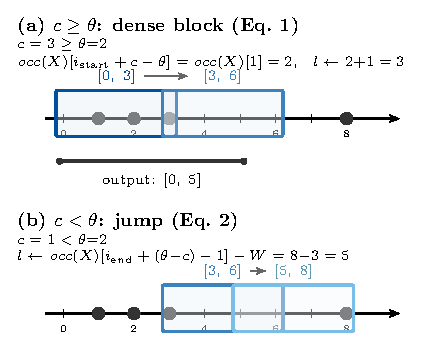
\includegraphics[width=\columnwidth]{fig/scan_stride.pdf}
\caption{Scan Stride Skipping の動作（式~\eqref{eq:stride_dense}，\eqref{eq:stride_sparse}）。}
\label{fig:scan_stride}
\end{figure}

\subsection{Apriori Interval Pruning}

古典的 Apriori~\cite{agrawal1994fast} の反単調性（anti-monotonicity）は
「頻出アイテムセットの任意の部分集合も頻出である」という性質であり、
対偶をとれば「ある部分集合が非頻出ならそのスーパーセットも必ず非頻出」となる。
本手法ではこれを\textit{区間単位}で適用する。
$Y \subseteq X$ ならば $X$ が時刻 $t$ に出現するときは常に $Y$ も出現するから、
任意のウィンドウ $[l, l+W]$ に対して
\[
  \mathrm{sup}(X, l, W) \leq \mathrm{sup}(Y, l, W)
\]
が成り立つ（補題~\ref{lem:apriori}、付録~C）。
すなわち $[l, l+W]$ が $Y$ の密集区間でなければ $X$ の密集区間にもなりえない。
よってサイズ $k$ の候補 $X$ が密集しうる左端 $l$ は、
全 $(k{-}1)$ 部分集合が密集する $l$ 値集合の共通部分に限定される：
\begin{equation}\label{eq:cand}
  R_X = \bigcap_{Y \subsetneq X,\, |Y|=k-1} \mathcal{T}_\theta(Y),
\end{equation}
ここで $\mathcal{T}_\theta(Y)$ は $Y$ が密集する左端の集合である。
$R_X$ に含まれない $l$ は安全にスキップでき、スキャン範囲を大幅に削減できる。


\subsection{$\Delta$-ステップストリーミング}

対象デプロイメントでは、イベントがセンサストリームまたは自律エージェントログから継続的に到着し
データベースに追記される。
システムは $\Delta$ 秒ごとにスキャンをトリガーする。

各スキャンステップは以下のように進行する：

\begin{enumerate}
  \item $\Delta$ 秒が経過したとき（現在位置 $s$）、バッファ $[s - W + 1,\; s + \Delta)$ を取得し、
        境界損失を防ぐため直前ステップから最新 $W{-}1$ 件のイベントを保持する。
  \item Scan Stride Skipping および Apriori Interval Pruning を適用した単調スキャンを
        このバッファに対して実行する。
  \item まだ出力していない $l_e + W \leq s$ を満たすすべての区間 $(X, [l_s, l_e])$ を出力する：
        これらは\textbf{確定}しており、将来のイベントによって変化しない。
  \item 次の $\Delta$ 件のイベント蓄積まで待機し、繰り返す。
\end{enumerate}
